\section{Results}\label{sec:results}
\subsection{Voltage controlled voltage source (VCVS)}\label{sec:vcvs}
A VCVS was constructed following the schematic in Fig. \ref{fig:schematics}\subref{fig:vcvs}. 
$\pm$10 V was used as supply voltage for the op amp.
The response of the output voltage to changes in input voltage is shown in Fig. \ref{fig:vcvs-graph}.

\begin{figure}[htpb]
	\centering
	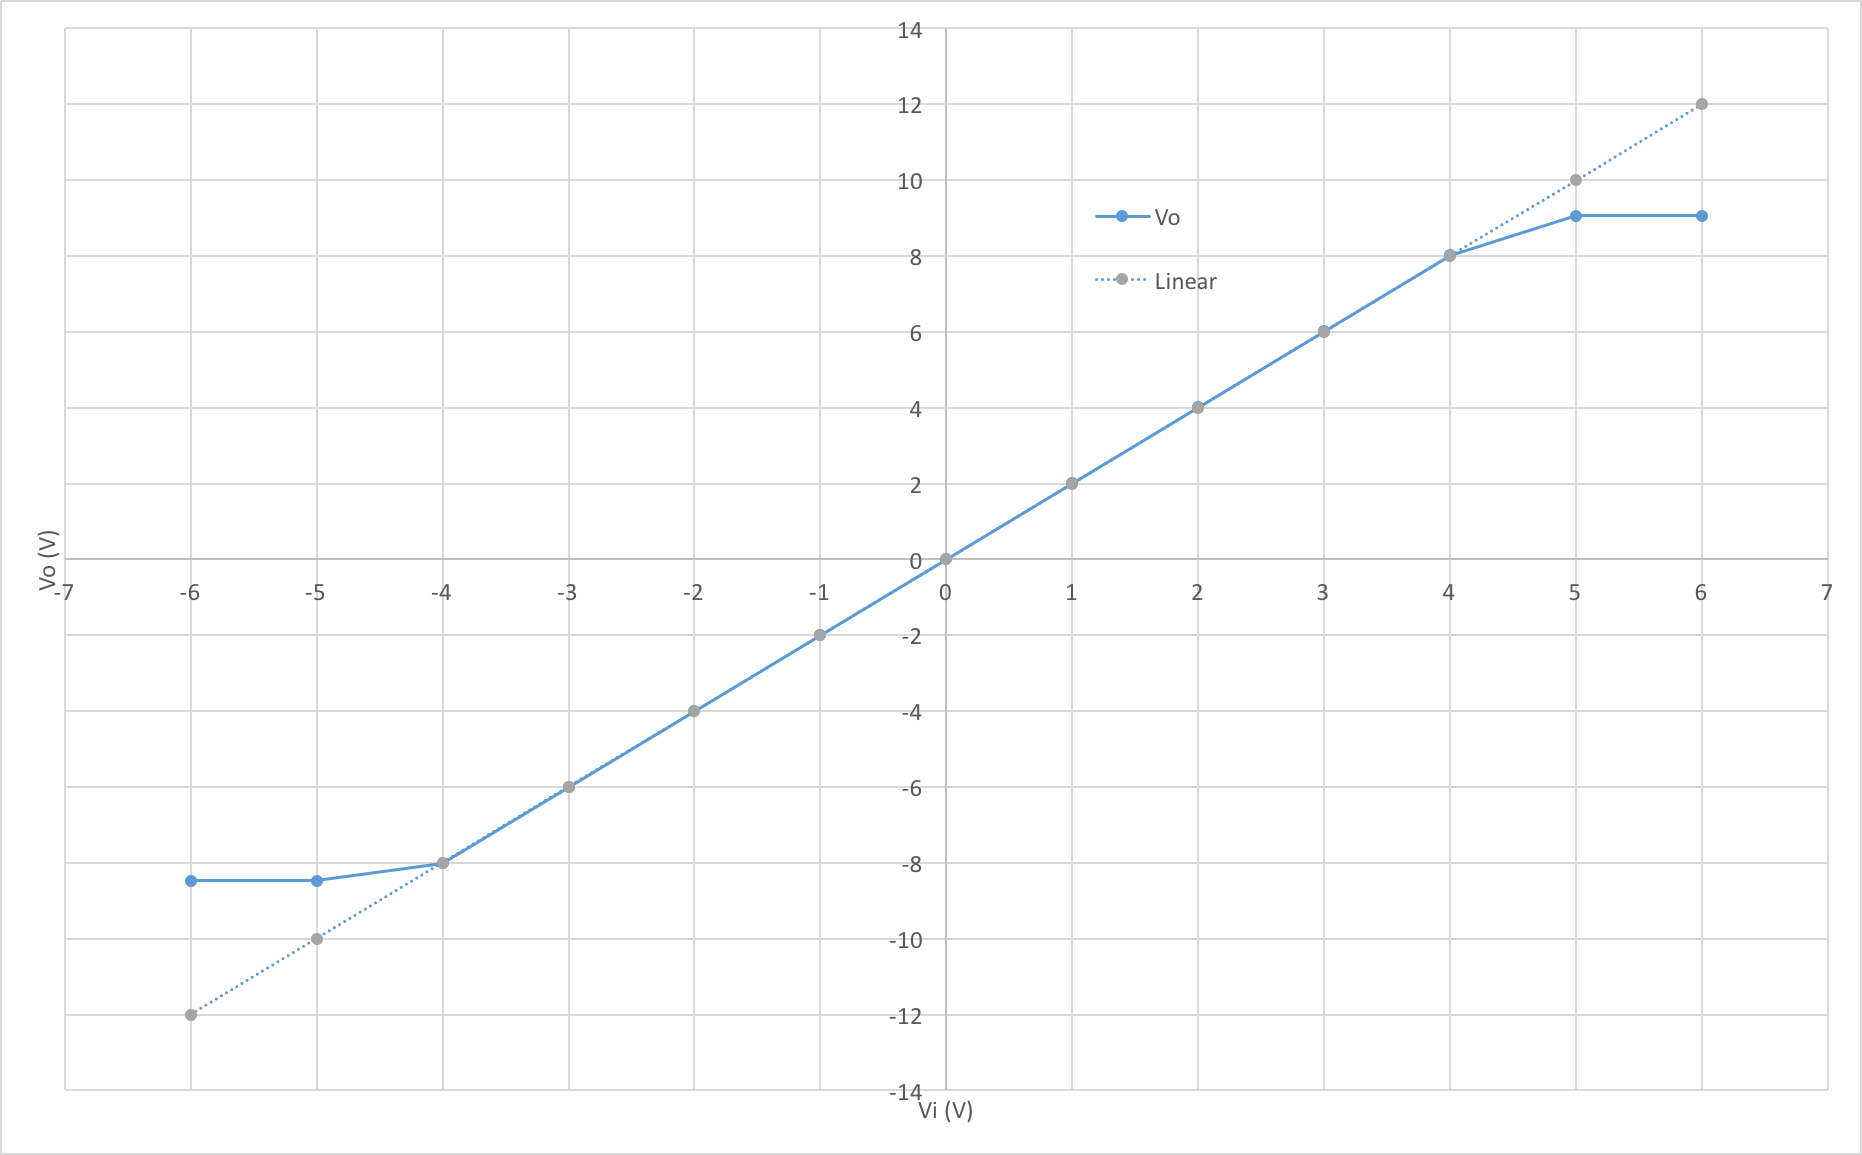
\includegraphics[width=0.95\linewidth]{graphics/vcvs-graph}
	\caption{Response characteristic of VCVS with expected linear behavior}
	\label{fig:vcvs-graph}
\end{figure}

\subsection{Voltage controlled current source (VCCS)}\label{sec:vccs}
A VCCS was constructed following the schematic in Fig. \ref{fig:schematics}\subref{fig:vccs}.
$\pm$10 V was used as supply voltage for the op amp.
The response of the output voltage to changes in input voltage is shown in Fig. \ref{fig:vccs-graph} for $R_L = \SI{1}{\kilo\ohm}$.

\begin{figure}[tbph]
	\centering
	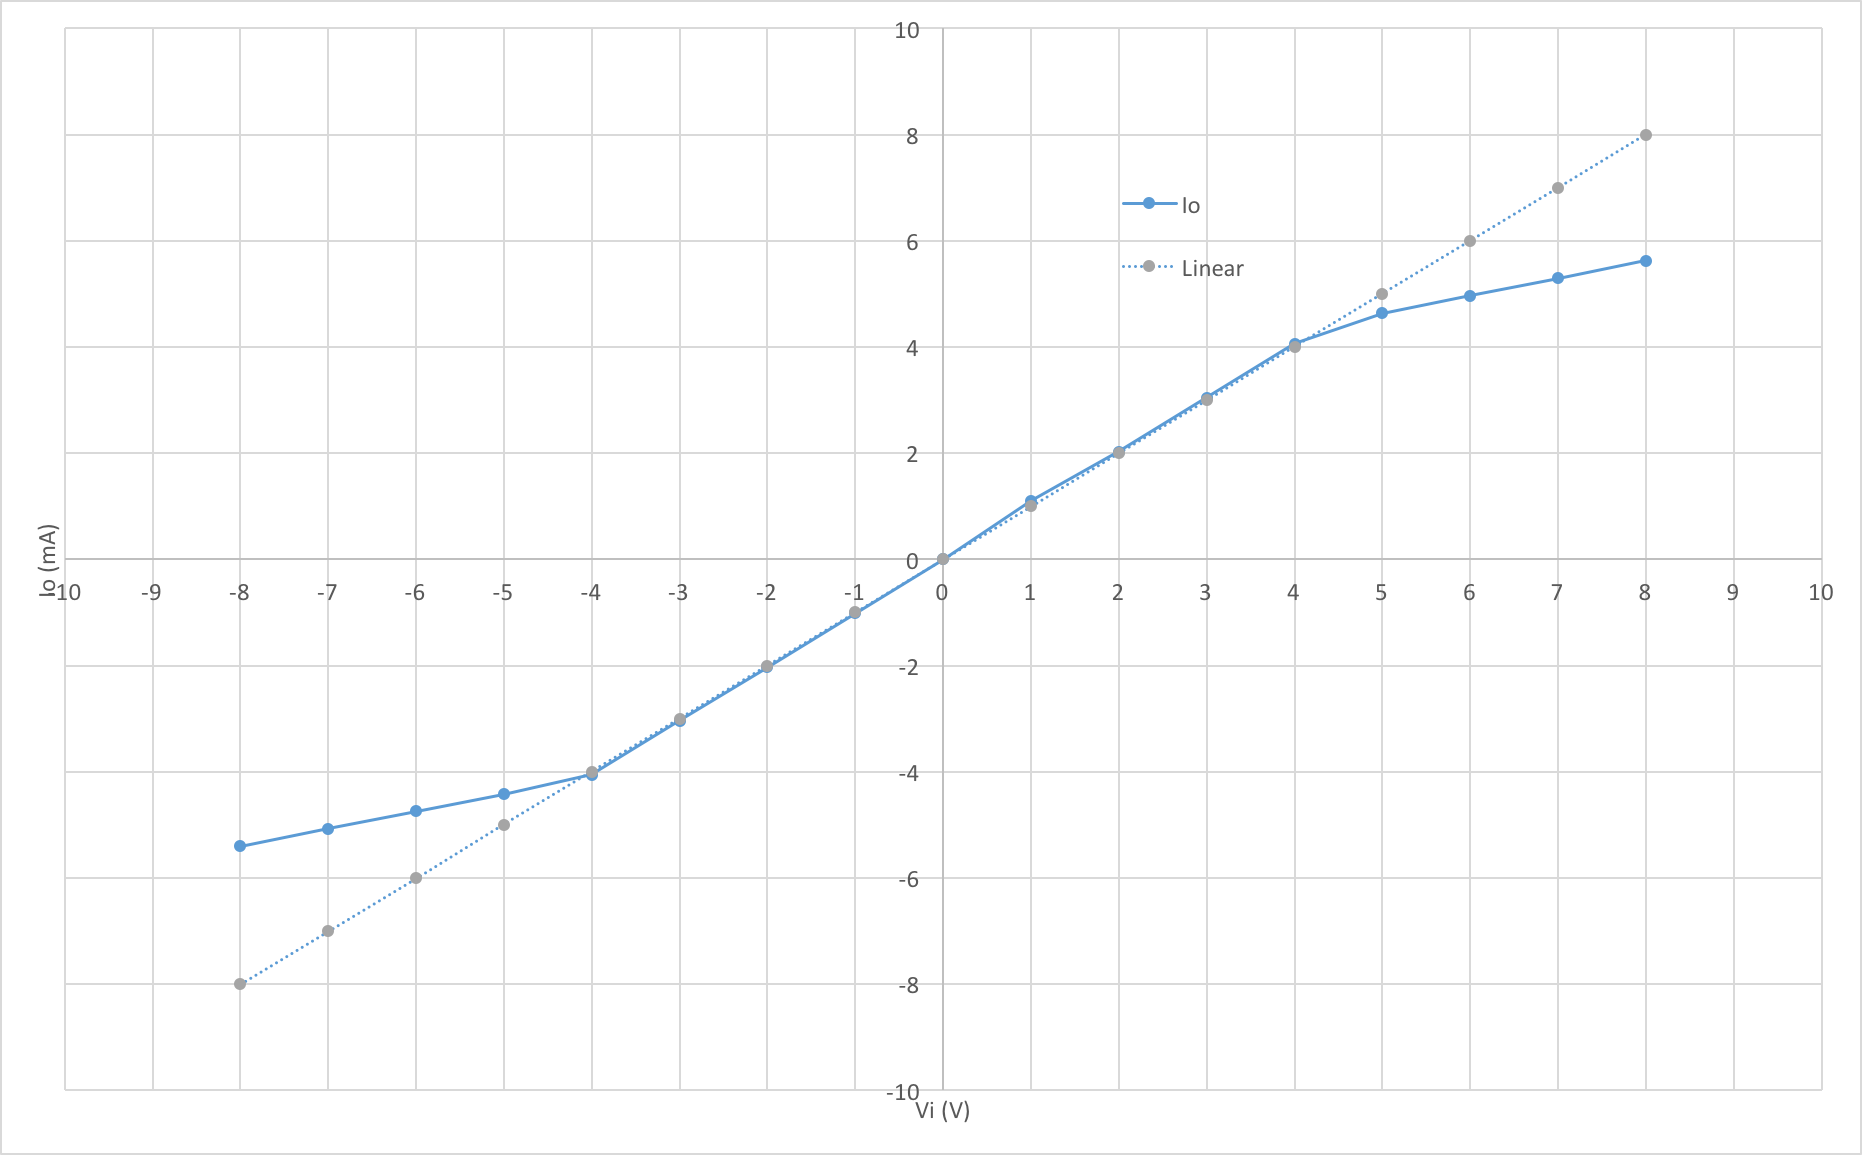
\includegraphics[width=0.95\linewidth]{graphics/vccs-graph}
	\caption{Response characteristic of VCCS with expected linear behavior}
	\label{fig:vccs-graph}
\end{figure}
